%%=======================================
%  WHUT Bachelor Thesis v 0.1b
%  
%  Tsao Yu
%  tsaoyu@tsaoyu.com
%  Last Modify Date Feb.6,2014
%%=======================================
\documentclass[cs4size,a4paper]{ctexart}   
%==================== 数学符号公式 ============
\usepackage{amsmath}                 % AMS LaTeX宏包
%\usepackage{amssymb}                % 用来排版漂亮的数学公式
%\usepackage{amsbsy}
\usepackage[style=1]{mdframed}
\usepackage{amsthm}
\usepackage{amsfonts}
\usepackage{mathrsfs}                % 英文花体字 体
\usepackage{bm}                      % 数学公式中的黑斜体
\usepackage{bbding,manfnt}           % 一些图标,如 \dbend
\usepackage{lettrine}                % 首字下沉,命令\lettrine
\def\attention{\lettrine[lines=2,lraise=0,nindent=0em]{\large\textdbend\hspace{1mm}}{}}
\usepackage{longtable}
\usepackage[toc,page]{appendix}
\usepackage{geometry}                % 页边距调整
\geometry{top=3.0cm,bottom=2.7cm,left=2.5cm,right=2.5cm}
%\usepackage{relsize}                % 调整公式字体大小:\mathsmaller,\mathlarger
%\usepackage{caption2}               % 浮动图形和表格标题样式
%====================公式按章编号==========================
\numberwithin{equation}{section}
\numberwithin{table}{section}
\numberwithin{figure}{section}
%================= 基本格式预置 ===========================
\usepackage{fancyhdr}
\pagestyle{fancy}
\fancyhf{}  
\fancyhead[C]{\zihao{5}  \kaishu 武汉理工大学毕业设计(论文)}
\fancyfoot[C]{~\zihao{5} \thepage~}
\renewcommand{\headrulewidth}{0.65pt} 
\CTEXsetup[format={\centering\bfseries\zihao{-2}},name={第, 章}]{section}
\CTEXsetup[nameformat={\bfseries\zihao{3}}]{subsection}
\CTEXsetup[nameformat={\bfseries\zihao{4}}]{subsubsection}
%================== 图形支持宏包 =========================
\usepackage{subfigure}
\usepackage{graphicx}                % 嵌入png图像
\usepackage{color,xcolor}            % 支持彩色文本、底色、文本框等
\usepackage{hyperref}                % 交叉引用
\usepackage{caption}
\captionsetup{figurewithin=section}
%==================== 源码和流程图 =====================
\usepackage{listings}                % 粘贴源代码
\usepackage{tikz}                    
\usepackage{tikz-3dplot}
\usetikzlibrary{shapes,arrows,positioning}
%===================   正文开始    ===================
\begin{document}
\bibliographystyle{gbt7714-2005}     %论文引用格式
%===================  定理类环境定义 ===================
\newtheorem{example}{例}              % 整体编号
\newtheorem{algorithm}{算法}
\newtheorem{theorem}{定理}            % 按 section 编号
\newtheorem{definition}{定义}
\newtheorem{axiom}{公理}
\newtheorem{property}{性质}
\newtheorem{proposition}{命题}
\newtheorem{lemma}{引理}
\newtheorem{corollary}{推论}
\newtheorem{remark}{注解}
\newtheorem{condition}{条件}
\newtheorem{conclusion}{结论}
\newtheorem{assumption}{假设}
%==================重定义 ===================
\renewcommand{\contentsname}{目录}     
\renewcommand{\abstractname}{摘要} 
\renewcommand{\refname}{参考文献}     
\renewcommand{\indexname}{索引}
\renewcommand{\figurename}{图}
\renewcommand{\tablename}{表}
\renewcommand{\appendixname}{附录}
\renewcommand{\proofname}{证明}
\renewcommand{\algorithm}{算法} 
%============== 封皮和前言 =================
%===============  封面  =================
\smallskip
\begin{center}
\begin{figure}[!th]
\centering

\includegraphics[width=0.7\linewidth]{figure/SchoolName}
\end{figure}

\vspace*{1.0cm}
{\zihao{1} 毕业设计(论文)} \\
\vspace*{2.1cm}
 \heiti{\zihao{1} 心理测评系统的设计与实现 }\\
\vspace*{5.0cm}
\songti
\begin{tabular}{cc}
 \zihao{-2} 学院(系):&\underline{\makebox[7cm][c]{\zihao{-2}计算机科学与技术学院}} \\ 
 \\
 \zihao{-2}专业班级: & \underline{\makebox[7cm][c]{\zihao{-2}软件工程zy1501班}} \\ 
 \\
 \zihao{-2}学生姓名: & \underline{\makebox[7cm][c]{\zihao{-2}吕世豪}} \\ 
 \\
 \zihao{-2}指导教师: & \underline{\makebox[7cm][c]{\zihao{-2}刘传文}} \\ 
 \\
\end{tabular} 
\end{center}
\thispagestyle{empty}
\clearpage
%=====================原创性声明===========
\begin{center}
\zihao{-2} \textbf{学位论文原创性声明}
\end{center}

本人郑重声明:所呈交的论文是本人在导师的指导下独立进行研究所取得的研究成果。除了文中特别加以标注引用的内容外,本论文不包括任何其他个人或集体已经发表或撰写的成果作品。本人完全意识到本声明的法律后果由本人承担。 
\begin{flushright}
\zihao{4} 作者签名:\qquad ~~~\\

年\qquad 月\qquad 日
\end{flushright}
\vskip 2cm
\begin{center}
\zihao{-2} \textbf{学位论文版权使用授权书}
\end{center}

本学位论文作者完全了解学校有关保障、使用学位论文的规定,同意学校保留并向有关学位论文管理部门或机构送交论文的复印件和电子版,允许论文被查阅和借阅。本人授权省级优秀学士论文评选机构将本学位论文的全部或部分内容编入有关数据进行检索,可以采用影印、缩印或扫描等复制手段保存和汇编本学位论文。\smallskip

本学位论文属于
\begin{tabular}[t]{l}
1、保密$ \Box$,在~~~年解密后适用本授权书  \\ 
2、不保密$ \Box$  \\ 
\end{tabular} \\
\begin{center}
(请在以上相应方框内打“$\surd”$)
\end{center}
\begin{flushright}
\zihao{4} 作者签名:  \quad\quad\quad\quad 年 \quad  月  \quad  日\\
导师签名:   \quad\quad\quad\quad 年 \quad  月 \quad   日\\
\end{flushright}
\thispagestyle{empty}
\clearpage

%%=============设计(论文)任务书===========
%\begin{center}
%\zihao{-2}\textbf{\songti 本科生毕业设计(论文)任务书} 
%\end{center}
%\smallskip
%\renewcommand{\arraystretch}{1.3}
%\begin{tabular}{lll}
%\zihao{4} \textbf{\songti 学生姓名: 曹宇} & & \zihao{4} \textbf{\songti 专业班级:\quad\quad 船海1006班} \\ 
%\zihao{4} \textbf{\songti 指导教师:徐海祥}&\makebox [3cm] & \zihao{4} \textbf{\songti 工作单位:\quad 武汉理工大学} \\ 
%\end{tabular}\\
%\begin{tabular}{lll}
%\zihao{4} \textbf{\songti 设计(论文)题目:}& \zihao{4} \textbf{\songti  武汉理工本科论文\LaTeX 模板 } &\\ 
%\zihao{4} \textbf{\songti 设计(论文)主要内容:} \\
%\end{tabular} \\ 
%\begin{enumerate}
%\item \LaTeX 环境的配置
%\item 主要字体的控制和数学公式的选用
%\item 图表和代码的粘贴
%\end{enumerate}
%\begin{tabular}{ll}
%\zihao{4} \textbf{\songti 要求完成的主要任务:}
%\end{tabular} \\ 
%\begin{enumerate}
%\item 选择合适的\TeX 编辑系统
%\item 学习如何使用控制代码完成排版
%\item 合理的安排学习和科研的时间来发展自己兴趣爱好
%\end{enumerate}
%\begin{tabular}{ll}
%\zihao{4} \textbf{\songti 必读参考资料:}
%\end{tabular}
%\begin{enumerate}
%\item \LaTeX  \quad User Manual
%\item  字体设计的艺术
%\end{enumerate}
%\begin{tabular}{lll}
%\zihao{4} \textbf{\songti 指导教师签名: }&\makebox [4cm]& \zihao{4} \textbf{\songti 系主任签名:} \\
%& & \zihao{4} \textbf{\songti 院长签名(章)}
%\end{tabular}
%\thispagestyle{empty}
%\clearpage
%%==========本科生毕业设计(论文)开题报告  =============
%\begin{center}
%\zihao{-2} \textbf{\songti 武汉理工大学}\\
%\zihao{-2} \textbf{\songti 本科生毕业设计(论文)开题报告} 
%\end{center}
%\begin{tabular}{|l|}
%\hline \rule[-2ex]{0pt}{5.5ex} \makebox[13.5cm][l]{\zihao{4} \heiti 1、目的及意义(含国内外的研究现状分析) } \\ 
%\quad \LaTeX 是国际通行的科技论文排版软件,国际上科研机构和大学都采用它写作\\
%\quad 国内著名高校都有自己的本科生\LaTeX 模板供毕业生使用\\
%\quad 但是武汉理工大学还没有本科生\LaTeX 模板可以参考\\
%\quad 人类的价值在于创造而不是索取 \\
%\hline \rule[-2ex]{0pt}{5.5ex}  \zihao{4} \heiti
%2、基本内容和技术方案\\ 
%\quad 采用GITHUB托管降低代码维护成本\\
%\quad 加入在线\TeX 编辑器的使用简介 \\
%\quad 授人以渔,注重方法和理念的引导\\
%\hline \rule[-2ex]{0pt}{5.5ex}  \zihao{4} \heiti
%3、进度安排 \\ 
%\quad 离 deadline 两个月吃喝玩乐 \\
%\quad 离 deadline 一个月吃喝玩乐 \\
%\quad 离 deadline 半个月吃喝玩乐 \\
%\quad 离 deadline 一个星期狂写论文 \\
%\hline \rule[-2ex]{0pt}{5.5ex} \zihao{4} \heiti
%4、指导教师意见 \\ 
%\quad 曹宇同学是个好同志\\
%\quad 曹宇同志是个好同学\\
%\quad 本表格是支持跨页的长表格,你可以复制上面的内容进行测试\\
%\quad 具体方法是将tabular改为 longtable然后再编译\\
%\makebox[10cm][r]指导教师签名:\\
%\makebox[12cm][r]\quad 年\quad 月\quad 日\\
%\hline 
%\end{tabular} 
%\thispagestyle{empty}

\pagestyle{plain}
\pagenumbering{Roman}
\section*{\zihao{2} \centering 摘要}

\vskip0.5cm
心理评测是一种比较先进的测试方法,它是指通过一系列手段,将人的某些心理特征数量化,来衡量个体心理因素水平和个体心理差异差异的一种科学测量方法。按评测的内容、对象特点、表现形式、目的、时间、要求等分为若干种类。主要是各机关、企业、组织等用来选拔人才、安置岗位以及对一个人进行诊断、评价、辅助咨询的一种手段,心理测评包含能力测试、人格测试和兴趣测试等。

本论文实现了一个B/S架构的心理评测系统,基于Python的flask框架,React框架和MySQL数据库,实现了用户的注册登录、账号激活、找回密码、管理员管理试卷、管理员管理用户、计算分数、分析答案得出结论的功能。

使用系统可以进行心理评测并得出结论,每份试卷针对性的让使用者了解自己对应指标的分数,更加了解自己对应方面的优点和缺点,同时也使管理员能够根据成绩进行筛选用户,了解大众的心理趋势。


\textbf{关键词:}  心理评测,结果分析,档案管理,目标筛选
\addcontentsline{toc}{section}{摘要}

\clearpage
\section*{\zihao{2} \centering \textbf{Abstract} }
   %用了Times New Roman字体来美化观感

Psychological assessment is a relatively advanced testing method. It refers to a scientific measurement method to measure the level of individual psychological factors and individual psychological differences by quantifying some psychological characteristics of human beings through a series of means. According to the content, object characteristics, manifestation, purpose, time and requirements of the evaluation, it can be divided into several categories. It is mainly a means used by various organs, enterprises and organizations to select talents, place posts, diagnose, evaluate and assist a person in counseling. Psychological assessment includes ability test, personality test and interest test. Generally speaking, psychological assessment has great significance in education, society and work. This system completes the basic function of psychometric assessment.

This paper implements a psychological evaluation system based on B/S architecture. Based on Python flask framework, React framework and MySQL database, the functions of user registration, account activation, password retrieval, administrator management test paper, administrator management user, calculating scores, analyzing answers and drawing conclusions are realized.

The system can be used to carry out psychological evaluation and draw conclusions. Each test paper aims to let users know their corresponding index scores, better understand the advantages and disadvantages of their corresponding aspects. At the same time, administrators can screen users according to their scores and understand the psychological trends of the public.

\textbf{Key Words:} Psychological assessment, Result analysis, File management, Target selection \\
\addcontentsline{toc}{section}{Abstract}





\pagestyle{empty}
\tableofcontents 
\thispagestyle{empty}
%============== 论文正文   =================
\pagestyle{fancy}
\pagenumbering{arabic}
\section{需求分析}

心理评测是一种比较先进的测试方法,它是指通过一系列手段,将人的某些心理特征线性化,衡量个体心理因素水平和个体心理差异的一种科学测量方法。按评测的内容、对象特点、表现形式、目的、时间、要求等分为若干种类。主要是各机关、企业、组织等用来选拔人才、安置岗位以及对一个人进行诊断、评价、辅助咨询的一种手段,心理测评包含能力测试、人格测试和兴趣测试等。

\subsection{心理测评的意义}

\subsubsection{心理评测在社会中的意义}

(1) 描述:心理评测可以从个体的智力、能力倾向、创造力、人格、心理健康等各方面对个体进行全面的描述,说明个体的心理特性和行为。

(2) 诊断:心理评测可以对同一个人的不同心理特征间的额差异进行比较,从而确定其相对优势和不足,发现行为变化的原因,为决策提供信息。 

(3) 预测:心理测评可以确定个体间的差异,并由此来预测不同的个体在将来的活动中可能出现的差别,或推测个体在某个领域未来成功的可能性。 

(4) 评价:可以评价个体在学习或者能力上的差异,人格的特点以及相对长处和弱点,评价儿童达到的发展阶段等。 

(5) 选拔:心理评测可以客观、全面、科学、定量化地选拔人才。 

(6) 安置:了解个体的能力、人格、心理健康等心理特征,从而为因材施教或人尽其才提供依据。 

(7) 咨询:心理测评可以为学校的升学就业咨询提供参考,帮助学生了解自己的能力倾向和人格特征,确定最有可能成功的专业或者职业。 

\subsubsection{心理测评在理论研究中的意义}

(1) 搜集资料:心理测评是搜集有关心理学资料的一个简单易行而又可靠的方法。

(2) 建立和检验假设:从心里测评的资料中可以发现问题,建立理论假设,并且可通过测量结果进一步来检验这些假设,进而推动心理科学的发展,例如智力结构理论的提出和发展,智力测验就起了重要作用。

\subsubsection{心理测评在教育领域中的意义}

(1) 心理测评是教学和学习的优良工具:通过心理评测教师和学生可以了解自己的心理状态,教师对学生的心里评测结果可以进行分析,改善自己的教学方法,学生能从自己的心里评测报告改善自己的生活习惯、思考方式和学习方式。老师可以做到因材施教,学生可以找到自己适合的学习方式。

(2) 心理测评创新教育的重要手段:收集学生们的心里评测结果,可以对当前教育形式做出判断,从而改善教育结构和方针,修正未来教育的路线,改进整个社会教育的结构。

\subsection{国内外心理评测现状分析}

国外发达国家对心理健康问题的研究起步早,发展力度大,早已形成了比较健全和成熟的心理健康服务体制。以美国为例,高校心理辅导人员配比较为充足,并且从事心理咨询工作的人员呢必须达到由APA和NASP两个专业组织制定规定的专业水平才有资格从业。并且由于在较早的年龄阶段就开始关注公民的心理健康,所以公民可以把接受心理治疗与身体治疗同等看待,这都使得线上面对面式的心理综合测评较为容易实施。

但是我国对心理问题的关注,起步晚,发展慢,国家投入与学科支撑还不足够,也没有充足的相关从业人员,各地的心理健康服务机构也并不完善。需要进行心理测评的用户分布广散,很难进行集中的测试。更为重要的是,由于目前我国在此方面的宣传与指导缺乏,许多人不愿意接受直接的心理咨询与辅导,这就使得很难有机会进行线下的心理测评。基于这些现实情况,使用计算机线上评测能够减少地域上带来的不便和隐私问题,保护用户的隐私可以让用户在做评测时候更加的真实,让测量结果更加准确。

常用的心里评测需要进行多套经典量表才能全面评估个体心理状况,存在诸多的局限。当题量大的时候,根据不完整调查,15\% 的受测者会出现疲劳、烦躁等不良情绪,进行 30 分钟的时候,24\% 受测者会出现不良情绪,造成测评的效率低。多套量表的设定还会出现维度重复甚至产生不需要测评的维度的问题,造成测评资源的重复和浪费。这也会影响后期数据的录入和清理,浪费大量时间和人力成本。

\subsection{需求分析}

\subsubsection{功能性需求}

(1) 用户进行注册登录,系统保存用户信息并对密码进行加密存储。

(2) 用户可以查看并修改自己的个人信息。

(3) 用户进行心理测评,即可完成系统所要求完成的题目。

(4) 用户可以在完成测评后可以获取到分数和图表形式的测评结果。

(5) 管理员对试卷进行相关操作,例如查看、上传、管理。

(6) 管理员可以对用户进行批量管理与权限设置。

(7) 管理员可以根据成绩进行筛选分类,按照某些标准进行划分。

\subsubsection{非功能性需求}

(1) 页面响应迅速,不会出现白屏等情况。

(2) 对于难以表述的题目,可选择使用图片、音频等方式进行辅助。

(3) 保护用户隐私,避免个人隐私信息的泄露。

(4) 用户可在疲倦时暂停答题,系统将对已答部分进行保存,下次进入时可选择继续完成。

(5) 整体设计友好温和,尽量不给受测者压力,保障测评结果尽量少受外界因素的干扰。

\subsection{系统目标}

目前网络上较为流行的各类网页式心理测试又存在不系统不完整、信息无法储存、无法管理、无法对比查看、试卷来源不可靠、风险性较高、测试结果不详细没有指导意义等问题。该类测试随机性较大,传播速度快,传播范围广,但是受测者经过一次测试后很难重复测试持续跟踪,也就是说测试结果很难真正的给予受测者实质性的评判依据和进一步的指导,仅仅是停留在非常表面的随手答题阶段。

基于以上客观现实和待解决问题,本次毕设希望做到,每个人可以根据我们系统的分析结果了解当前自己的心理状态,明确自己的目标,改进自己的不足,使得心理测评系统真正的产生实质性功效。      %
\section{系统设计}

\subsection{总体设计}

\subsubsection{功能设计}

\begin{figure}[thbp!]
	\centering
	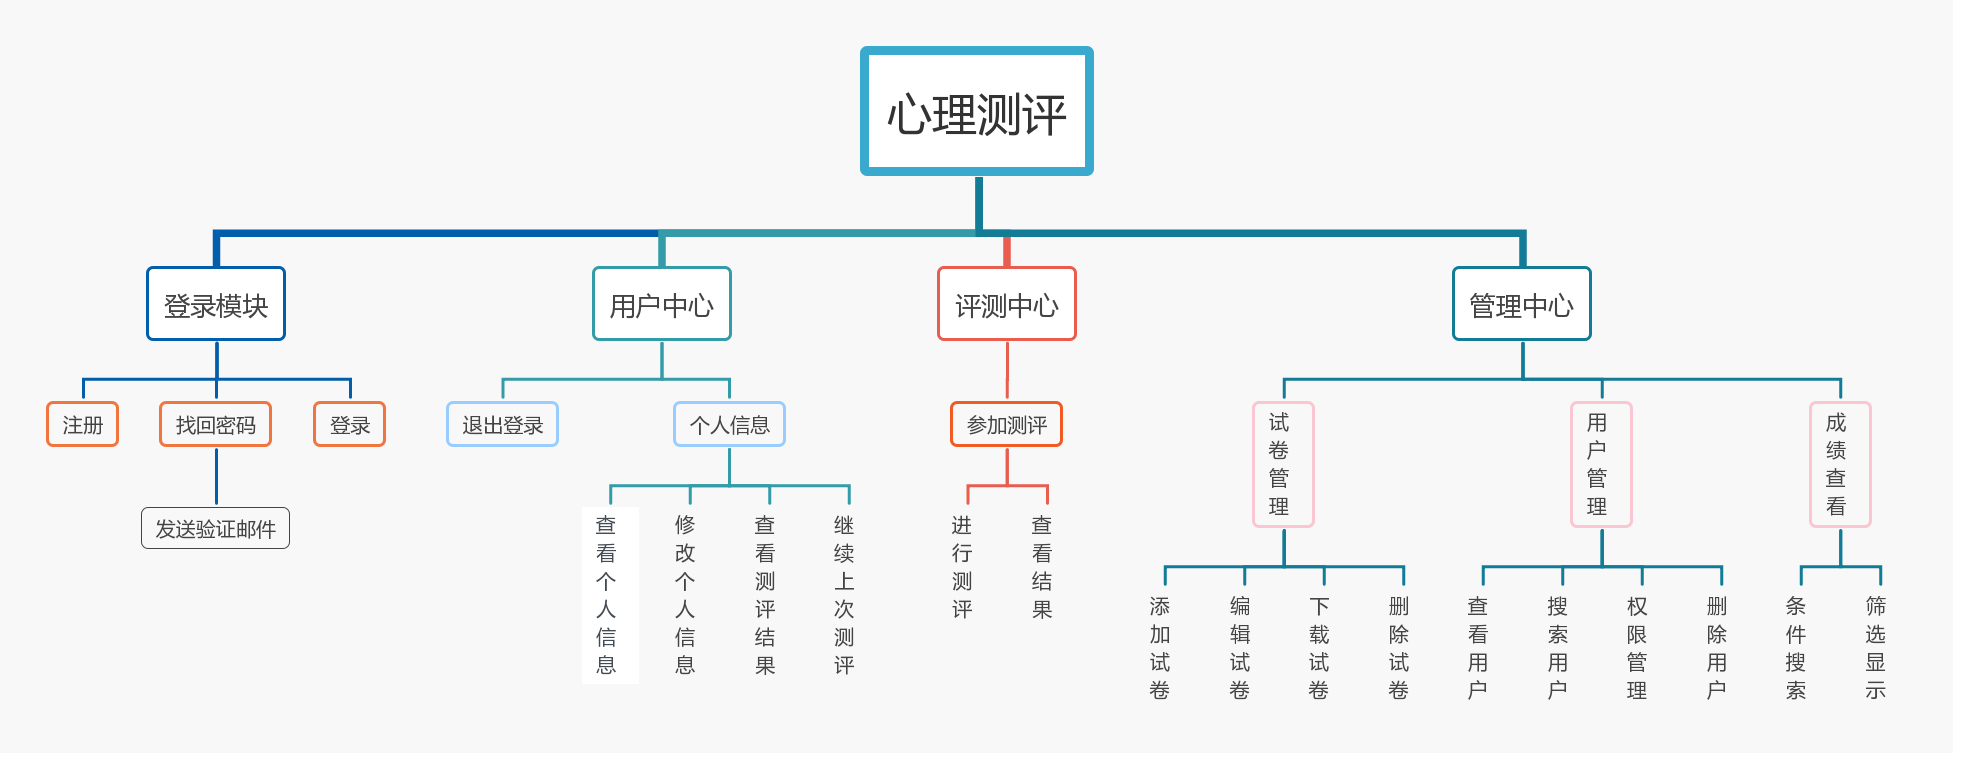
\includegraphics[width=1.0\linewidth]{figure/functions}
	\caption{系统功能设计}
	\label{fig:functions}
\end{figure}

心理评测系统由登陆模块、用户中心、评测中心和管理中心四大模块组成。登陆模块涉及用户的注册、登陆、邮箱验证、找回密码四个功能。用户中心可以修改个人信息、查看已经做的试卷的测评结果、查看未完成试卷的进度。评测中心可以做试卷进行评测和查看结果。管理中心是管理员对试卷、用户、成绩进行管理的模块。

\subsubsection{用例设计}

\begin{figure}[htp]
	\centering
	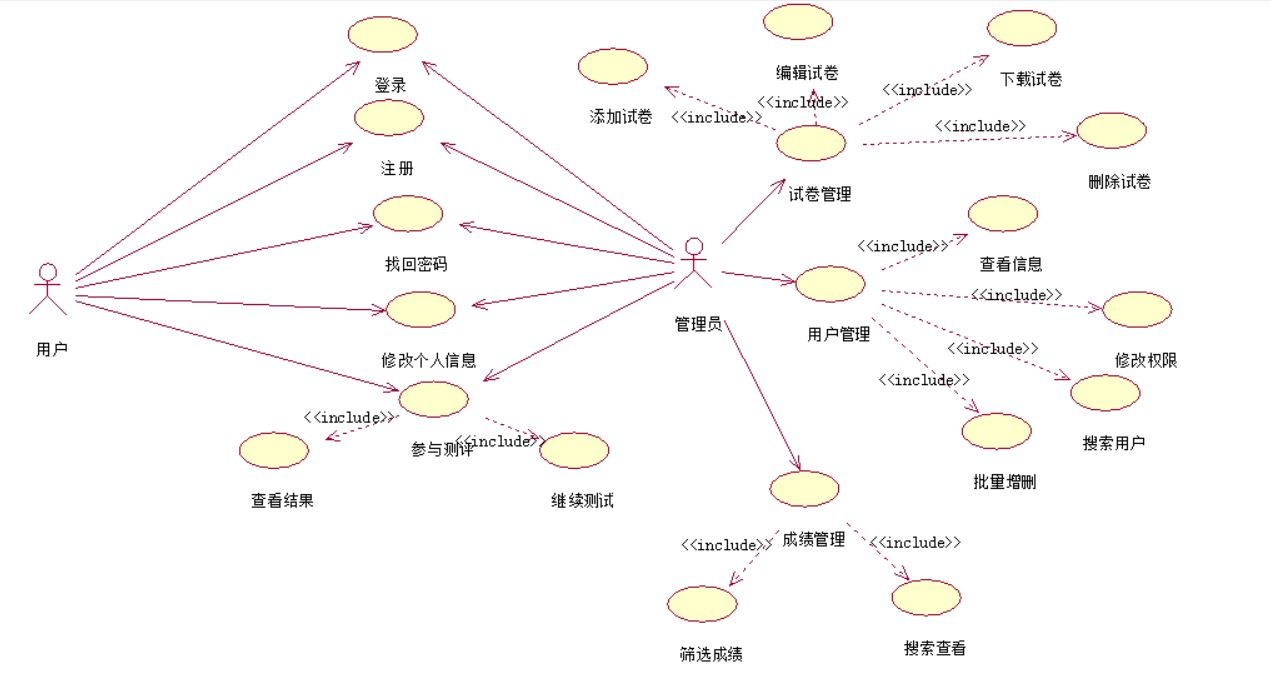
\includegraphics[width=0.8\linewidth]{figure/user_case}
	\caption{系统用例图}
	\label{fig:user_case}
\end{figure}

心里评测系统的用户分为两种类型:用户和管理员,其中管理员可以进行所有用户的操作,并且可以进入管理界面对试卷、用户、成绩进行管理。

\subsubsection{流程设计}

\begin{figure}[thbp!]
	\centering
	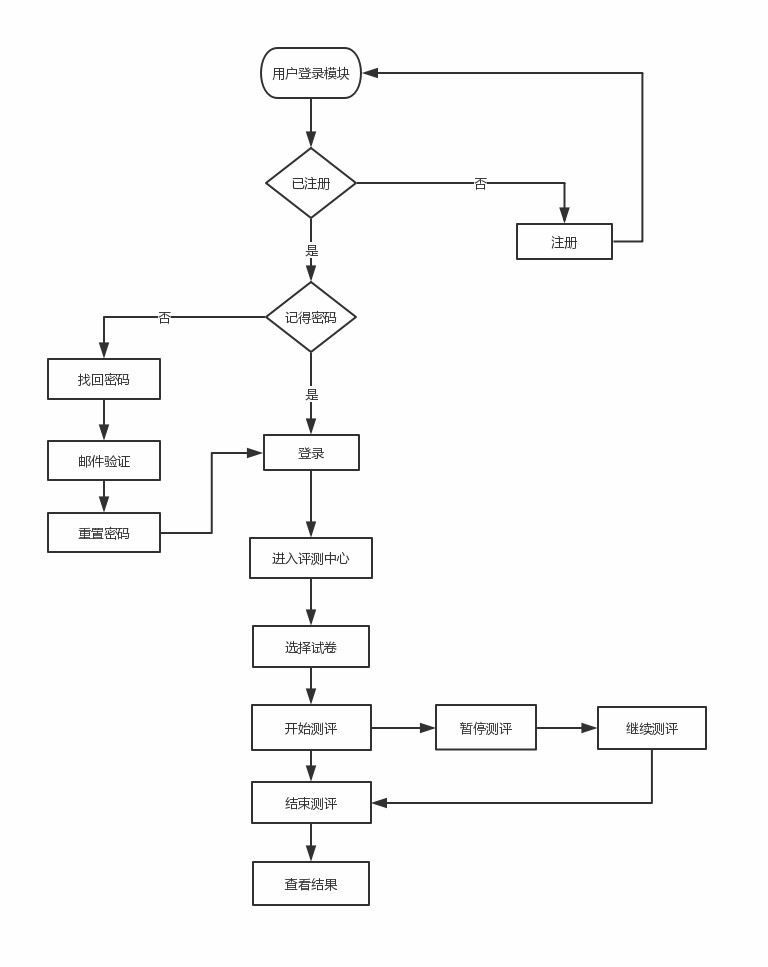
\includegraphics[width=0.8\linewidth]{figure/user_use}
	\caption{用户流程图}
	\label{fig:user_use}
\end{figure}

\begin{figure}[thbp!]
	\centering
	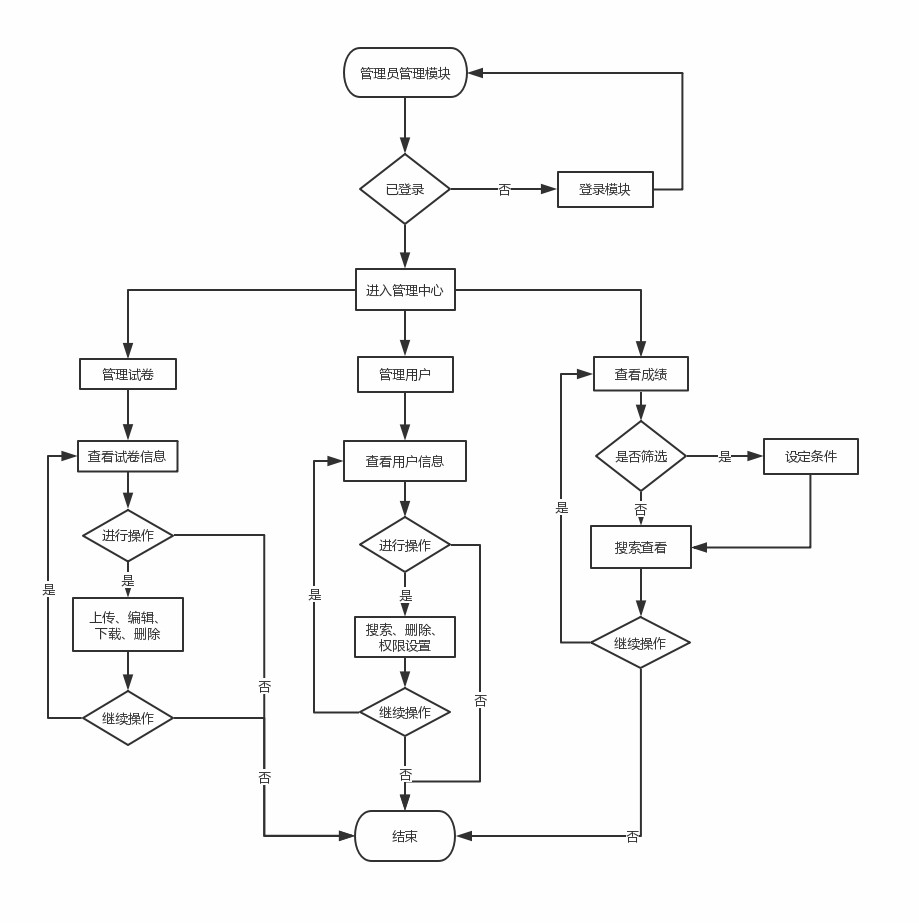
\includegraphics[width=1.0\linewidth]{figure/admin_use}
	\caption{管理员流程图}
	\label{fig:admin_use}
\end{figure}

\subsection{项目设计}

\subsubsection{前端项目架构}

\begin{figure}[thbp!]
	\centering
	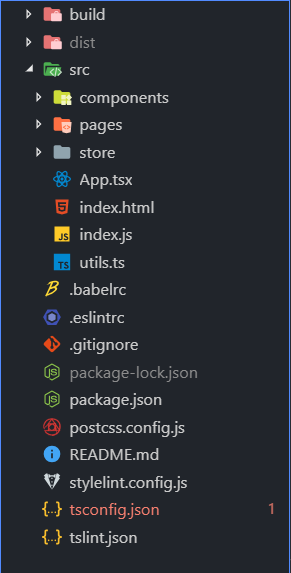
\includegraphics[width=0.3\linewidth]{figure/frontend_structure}
	\caption{前端项目目录}
	\label{fig:frontend_structure}
\end{figure}

build文件夹下存放着webpack的编译打包配置文件,分为两个环境,development开发环境和production生产环境。

dist文件夹是存放着webpack打包后的文件,用作于webpack-dev-server的开发环境文件和上线后的生产环境文件。

src文件夹是项目的根目录,里面的components文件夹存放着公用的组件,pages存放着系统的各个页面文件,store存放着项目所需要用到的redux状态仓库,App.tsx是项目的主页面,index.html是webpack打包注入js依赖的html文件,index.js是项目的主入口,utils.js是项目所需要的共用工具。

.babelrc是babel-loader的配置文件,配置编译js的目标版本。

.eslintrc是eslint代码检查的配置文件。

.gitignore是git仓库push的时候忽略的文件。

package.json是前端项目的架构文件,记载该前端项目所需要的依赖和依赖版本和该前端项目的基本信息。

postcss.config.js是postcss的配置文件。

README.md是描述该项目的markdown文件。

stylelint.config.js是stylelint css代码检查的配置文件。

tsconfig.json是Typescript的编译配置文件。

tslint.json是tslint的配置文件。

\subsubsection{后端项目架构}
\begin{figure}[thbp!]
	\centering
	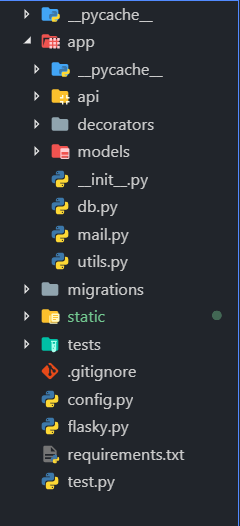
\includegraphics[width=0.3\linewidth]{figure/backend_structure}
	\caption{后端项目目录}
	\label{fig:backend_structure}
\end{figure}

\_\_pycache\_\_是IDE自动生成的sourcemap索引文件夹。

\_\_init\_\_.py文件是该Python包的默认包导出文件。

app文件夹是项目的根目录,api文件夹存放着Resuful API的文件,decorators文件夹存放着项目中所用到的装饰器,models文件夹存放着该项目所用到的所有对应数据库中的数据模型,db.py是该项目连接数据库获得数据库实例的文件,mail.py是该项目所使用到的邮箱模块,utils.py是该项目的工具库。

migrations是Flask-Migrate根据Sqlalchemy ORM数据模型定义进行数据库备份的文件夹。

static是该后端项目的静态文件存放目录。

tests是后端项目的测试文件存放目录。

.gitignore是git仓库索要忽略文件的声明文件。

config.py是该项目的配置文件。

flasky.py是该项目的主入口文件,启动文件。

requirements.txt记录着该项目的依赖和依赖版本。

\subsection{项目重要依赖}

\subsubsection{React}

React是一个声明式,组件化的前端框架。其使用Virtual DOM技术把应用状态和DOM分离开来,搭配Diff算法来最小颗粒的更新DOM,而这一切开发者都不需要关心,开发者只需要专注注意力在开发业务代码上。React拥有极丰富的生态,本项目中还使用了React-redux来进行redux状态仓库的管理。

\begin{lstlisting}[language=C]
class App extends Component {
  public componentDidMount() {
  	...
  }
  
  public render() {
	return (
	  <div>
	    this is App
	      <a onClick={this.onClick}>
	  </div>
	)
  }
	  
  private onClick = (e: ClickEvent) => {
    e.preventDefault();
    ...
  }
}
\end{lstlisting}

\begin{center}
	{\small React编写组件}
\end{center}

所有React组件都要继承React.Component,拥有React组件的生命周期,每个React组件需要实现一个继承父类的render方法,来控制组件如何进行渲染。

\subsubsection{Flask}

Flask是一个使用 Python 编写的轻量级 Web 应用框架。其 WSGI 工具箱采用 Werkzeug ,模板引擎则使用 Jinja2 。Flask使用 BSD 授权。Flask也被称为 “microframework” ,因为它使用简单的核心,用 extension 增加其他功能。Flask没有默认使用的数据库、窗体验证工具。本项目中使用了Flask-Migrate来进行数据库的备份,Flask-Mail来进行邮件的发送,Flask-SqlAlchemy来进行更加简单的操作SqlAlchemy。

\begin{lstlisting}[language=C]
@app.route("/index")
def Index():
	return "<h1>Hello, Index</h1>"
\end{lstlisting}

\begin{center}
	{\small Flask定义视图路由}
\end{center}

传给app.route的是一个路径字符串,该方法返回一个装饰器,装饰器装饰路由函数,每个路由函数返回一个页面或者数据。

\subsubsection{Typescript和Javascript}

项目使用的前端语言并非常规的Javascript而是它的超集——Typescript,其作为超集在绝对兼容Javascript代码的前提下,加入了许多静态语言所拥有的特性,比如接口、泛型、类型判断等等。Javascript作为脚本语言其灵活性和方便性为大家所称道,但是也由于其灵活性,前端代码的质量低下导致项目难以维护和扩展,Typescript就是解决Javascript严谨性而诞生的一门语言。Java作为世界上用途最广泛,使用人数最多的语言就是因为其严谨性得到了很多企业的偏爱,Typescript看起来80\%都和Java很相似,可以理解为在Javascript的基础上加了一层代码检查和提示。

\subsubsection{前端构建工具——Webpack}

浏览器的版本众多,浏览器与浏览器之间的内核有许多差异,这导致同一份代码可能在不同浏览器下的表现不同,通过人工的方式编写兼容代码会有很高的人力成本和时间成本。同时在以前的开发过程中,前端依赖后端导致前端开发与后端严重耦合,降低了开发效率。前端工程化时代的到来,让前端拥有自己的项目构建能力,同时还解决了不同浏览器之间的兼容问题,诞生了许多前端构件工具,Gul、Grunt、Webpack等等。其中Webpack是当下活跃度最高,最火热的前端构建工具。

Webpack最主要的两个功能是编译和打包。本项目所使用的React是使用JSX语法,不是浏览器默认可支持的语法,所以要将我们的前端代码编译成浏览器可识别的代码。Webpack最重要的两个概念就是loader和plugin,loader负责各种类型文件(.css,.js,.ts,.png......)的编译工作,可以将他们转化成目标浏览器的可识别文件,plugin则负责除了编译以外的所有工作,包括打包,体积优化,分离依赖等等。

\begin{lstlisting}[language=C]
{
  test: /\.jsx?$/,
  exclude: /node_modules/,
  use: ["babel-loader"]
},
{
  test: /\.tsx?$/,
  exclude: /node_modules/,
  use: [{
    loader: "ts-loader",
    options: {
      transpileOnly: true,
      getCustomTransformers: () => ({
          before: [
            require("ts-import-plugin")({
              libraryName: "antd",
              libraryDirectory: "es",
              style: "css"})
          ]
      }),
      compilerOptions: { module: "es2015" }
    }
  }]
}
\end{lstlisting}

\begin{center}
	{\small Webpack编译jsx和tsx文件成es5的配置}
\end{center}

Webpack还提供了前端可实时预览的热更新服务器————webpack-dev-server,该插件可以实时的检测项目文件的变化并重新编译和打包让浏览器的页面刷新。

Webpack打包体积优化也是一个深奥的学问。

Webpack在原始配置的情况下,因为是单页面应用,所以打包出来以后的bundle文件非常之大,高达4MB,这对于首屏加载是非常不利的,过长的白屏会流失很多的用户量,所以Webpack的优化也是一门学问。

常用的优化有以下几点:

(1) 配置optimization中的splitChunks选项,会根据依赖图对于多次依赖的包单独打包然后进行引用。

(2) 配置externals选项对于第三库在html文件中进行CDN引用,打包时候忽略该库。

(3) 使用uglifyjsPlugin对打包文件进行压缩。

(4) 使用懒加载进行加载组件和页面,react-loadable可以通过一个高阶组件包裹我们的异步组件使用import函数进行异步的加载组件,当加载成功的时候显示组件否则就加载Loading组件。

(5) 配置Gzip。

进行上面的优化以后,打包以后的文件按照路由和组件分成了十几个文件,最大的体积不超过400KB,减少了首屏加载的时间。

\subsubsection{Pandas}

Pandas是一个数据科学分析第三方库,可以方便的建立矩阵以及对矩阵中的数据进行各种数学运算和变换,在解析试卷和成绩分析的时候有很多使用。同时可以对矩阵中的数据进行清理和类型的转换。

\subsection{数据库设计}

通过SqlAlchemy我们可以方便的在数据库中创建一个表并生成记录,同时也可以方便的进行数据库操作,定义数据之间的关系,搭配Flask-Migrate还可以方便的进行数据库备份、恢复和回滚。

这个系统的主要有三个表,用户表(users),试卷表(papers),成绩表(grades),数据库实体之间的关系,箭头都代表一对多关系,粗体字体为必填字段。

\begin{figure}[thbp!]
	\centering
	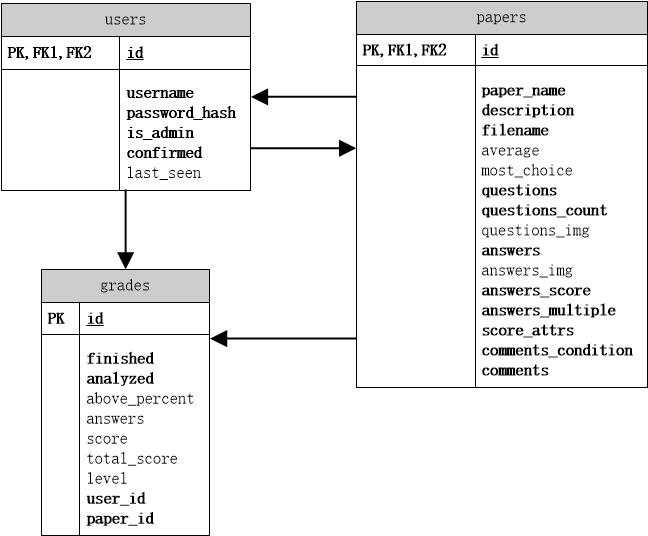
\includegraphics[width=0.7\linewidth]{figure/entity_relationship}
	\caption{数据库关系}
	\label{fig:entity_relationship}
\end{figure}

\subsubsection{一对多关系}

如图中,用户表和成绩表,试卷表和成绩表之间都为一对多关系。SqlAlchemy中可以方便的通过relationship和foreignKey进行设置一对多关系。

\begin{lstlisting}[language=C]
class User(Model):
...
grades = relationship("Grade", backref="user", lazy="dynamic",
cascade="all, delete-orphan", passive_deletes=True)

class Paper(Model):
...
grades = relationship("Grade", backref="paper", lazy="dynamic",
cascade="all, delete-orphan", passive_deletes=True)

class Grade(Model):
...
user_id = Column(Integer, ForeignKey("users.id",
ondelete="CASCADE"))
paper_id = Column(Integer, ForeignKey("papers.id",
ondelete="CASCADE"))
\end{lstlisting}

\begin{center}
	{\small 建立用户和成绩,试卷与成绩之间的一对多关系}
\end{center}

relationship的这一端代表着1的这一端,backref传入的是在Grade对象下如何访问User或者Paper对象,lazy代表如何访问这个对象,一对多之间的关系通过外键的形式进行设置,比如users.id代表着是users这张表中的id作为外键。同时外键的字段设置需要和做外键的字段类型一模一样,否则会报错。

(1) select,默认选项,直接查找出所有对象,例如user.grades直接通过列表列出所有该用户下的grade

(2) dynamic返回的是一个查询集,例如 users.grades.filter\_by(...)返回的是一个查询集可以进行筛选操作。

(3) joine类似于select,但是seletc在查询的过程中需要查询两个表,而joined是建立一个新的连结表进行查询,在数额大的情况下使用joined能节省不少性能。

\begin{center}
	{\small lazy选项}
\end{center}

SqlAlchemy作为最强大的ORM工具当然不只是定义关系,还有就是定义实体不存在的时候如何处理与其相关的数据,加入一个用户被删除了,那么于其关联的成绩也应该要全部删除,而不是作为冗余数据存在数据库中,一套试卷被删除了同理。那么cascade就是干这个事情的。

(1) save-update,默认选项,添加一条数据的时候会把其他和它相关的数据都添加到数据库中。

(2) merge,默认选项,合并一个对象的时候会将使用了relationship相关联的对象也进行merge操作。

(3) expunge,移除操作的时候,会将相关联的对象也进行移除,这个操作只是从session中删除,而不是从真正的数据库中删除。

(4) all,包含上面所有的选项。

(5) delete-orphan,删除相关的孤儿数据。

\begin{center}
	{\small cascade选项}
\end{center}

对应的要在多的那一端设置ondelete属性。

至此一对多的关系就设置好了,使用Flask-Migrate升级数据库的时候可以自动检测相关外键的设置然后更新数据库。

\subsubsection{多对多关系}

\begin{figure}[thbp!]
	\centering
	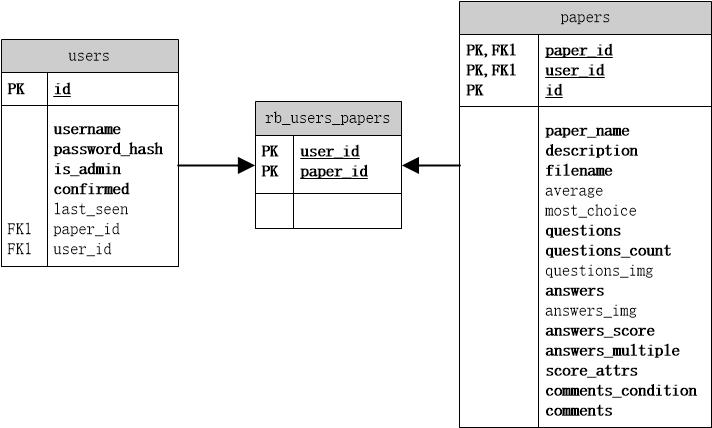
\includegraphics[width=1.0\linewidth]{figure/rb_users_papers}
	\caption{多对多关系}
	\label{fig:rb_users_papers}
\end{figure}

一个用户可以做多张试卷,一张试卷也可以有很多用户来做。这就是一个多对多关系。多对多关系中,需要一个额外的连接表来做查询。

\begin{lstlisting}[language=C]
class User(Model):
...
papers = relationship("Paper", secondary=rb_users_papers,
lazy="dynamic")

class Paper(Model):
...
users = relationship("User", secondary=rb_users_papers,
lazy="dynamic")

// 连接表
rb_users_papers = Table(
"rb_users_papers",
Column("user_id", Integer, ForeignKey("users.id"),
primary_key=True),
Column("paper_id", Integer, ForeignKey("papers.id"),
primary_key=True)
)
\end{lstlisting}

\begin{center}
	{\small 多对多关系代码}
\end{center}

上面的代码说明了users表和papers表之间是通过一个rb\_users\_papers进行连接查询的,同时连接表中的每个字段都需要与原字段的属性相同。在原表中的relationship中需要设置secondary属性来进行使用连接表的查询。使用连接表进行连接的两个表,任何一条记录被删除以后相关的连接表记录也会被删除,当然也可以设置与其关联的记录也被删除,但在此处的情况不适合这样做,试想一下,如果一个用户记录被删除了,那么该用户做过所有的试卷记录也会被删除,别人就无法做了,这样是非常的不合适的情况。

数据库的设计是一个完善的软件系统必备也是最重要的一个阶段,一个好的数据库设计能让一个系统的性能良好、易于维护、易于拓展。有些人可能会觉得直接手写sql更加灵活和方便,但是如果作为一个多人维护开发的系统来说,每个人都有自己写sql的习惯,会让项目代码水平层次不齐难于维护,这时候就要使用SqlAlchemy这种工具了,通过一种OOP的方式来进行数据库的管理。
\section{系统实现}

如果说一个项目的架构和数据库设计是一个项目的骨架,那么业务代码就是在其骨架上面生长的骨肉。一个好的骨架能够让血肉长的更加健康。

\subsection{前后端交互模型}

\subsubsection{RESTful API}

REST全称是Representational State Transfer,中文意思是表述(编者注:通常译为表征)性状态转移。 它首次出现在2000年Roy Fielding的博士论文中,Roy Fielding是HTTP规范的主要编写者之一。 他在论文中提到:"我这篇文章的写作目的,就是想在符合架构原理的前提下,理解和评估以网络为基础的应用软件的架构设计,得到一个功能强、性能好、适宜通信的架构。REST指的是一组架构约束条件和原则。" 如果一个架构符合REST的约束条件和原则,我们就称它为RESTful架构。

REST本身并没有创造新的技术、组件或服务,而隐藏在RESTful背后的理念就是使用Web的现有特征和能力, 更好地使用现有Web标准中的一些准则和约束。虽然REST本身受Web技术的影响很深, 但是理论上REST架构风格并不是绑定在HTTP上,只不过目前HTTP是唯一与REST相关的实例。 所以我们这里描述的REST也是通过HTTP实现的REST。

RESTful API有以下的特征:

\begin{enumerate}
	\item 每一个uri代表一种资源。
	\item 客户端和服务器之间,传递这种资源的某种表现层。
	\item 客户端通过四个HTTP动词(GET、POST、DELETE、PUT),对服务器端资源进行操作,实现"表现层状态转化"(增删改查)。
	\item URL中通常不出现动词,只有名词。
	\item 使用JSON不使用XML。
\end{enumerate}

\subsubsection{使用Redux存储网络请求状态}

Redux 是 JavaScript 状态容器,提供可预测化的状态管理。可以让你构建一致化的应用,运行于不同的环境(客户端、服务器、原生应用),并且易于测试。其使用Immutable数据结合React能让页面相应数据进行最小颗粒度的更新DOM结点。

因为Ajax都是异步的一个请求过程,需要在回调函数内对数据进行处理,这种就会出现当依赖的Ajax请求过多的情况下,不断的编写和嵌套回调函数的时候代码就会变得非常难以阅读和维护,所以使用Promise封装一种通用的Ajax API同时用Redux进行对数据的保存是非常有必要的。

当进行一个Ajax请求的时候,我们默认出发一个Redux Action将Ajax的数据储存在Redux中然后使用React-Redux的Connect函数将我们的组件根据Redux中的状态变化进行更新。

注意这里我们一定要在PromiseLike Function里面返回一个Promise对象来表示该Promise的状态,否则在使用Await关键字的时候,不会进行阻塞。

这样做的好处就是,通过封装了axios进行http请求的时候可以有一个公共的地方存储返回的数据,同时还可以在发生错误的时候或者在权限不够的时候读取headers直接取消渲染并给出提示让用户进行相应的操作。

\subsection{账号系统}

一个系统想要有人使用,给每个人都提供服务,都需要一个完善的账号系统,每个人都有自己的账号,进行登陆,使用系统,更改设置等等。

\subsubsection{密码加密}

出于安全考虑,用户的密码不通过明文保存,除非你对自己的运维系统有着极高的自信,当然这样也不建议这样做。毕竟人外有人,天外有天,如果没有被盗取那么说明你的系统价值还不是那么的高。

werkzeug.security是一个Python的密码包,其中的generate\_password\_hash的方法可以创建MD5加密的字符串,check\_password\_hash可以用于验证密码是否正确。

\begin{lstlisting}[language=C]
@property
def password(self):
raise TypeError("cannot read a user's password")

@password.setter
def password(self, password):
self.password_hash = generate_password_hash(password)

def verify_password(self, password):
if not password:
return False
return check_password_hash(self.password_hash, password)
\end{lstlisting}

\begin{center}
	{\small 用户密码的创建和验证}
\end{center}

\subsubsection{token的创建和验证}

token用于用户的登陆状态的保存,其通过cookie的形式保存在request头中,后端通过对response的set-cookie字段对网页的该域下进行cookie的设置。同时token可以设置过期时间。

\begin{lstlisting}[language=C]
def generate_confirm_token(self):
s = Serializer(current_app.config["SECRETE_KEY"],
expires_in=60 * 5, salt=current_app.config["CONFIRM_TOKEN"])
token = s.dumps({"user": self.username})
return token.decode()
\end{lstlisting}

\begin{center}
	{\small 得到加密token的代码}
\end{center}

初始化对象的时候向Serializer内部传入解密字符串,token的有效时长,以及加密的盐。此token的时长是五分钟,将用户的用户名做了加密通过HTTP传给前端,这里要注意,因为token生成的是二进制字符串,我们先要把它解密成普通字符串以后才能设置cookie,前端下次请求的时候会带上这个数据,后端再进行解密即可获得用户的状态。

\begin{lstlisting}[language=C]
response.set_cookie("token", token, max_age=max_age, 
httponly=True)
\end{lstlisting}

\begin{center}
	{\small response设置header中的cookie}
\end{center}

\begin{lstlisting}[language=C]
s = Serializer(current_app.config["SECRETE_KEY"], 
salt=current_app.config["CONFIRM_TOKEN"])
try:
data = s.loads(token)
if username != data["user"]:
return -2, "Bad signature"
return 0, "Confirm success"
except SignatureExpired:
return -1, "Signature expired"
except BadSignature:
return -2, "Bad signature"
\end{lstlisting}

\begin{center}
	{\small 验证token的代码}
\end{center}

同样的,在解密的过程中需要获得Serializer的实例,当loads一个token的时候,如果验证失败或者token超时,代码会抛出异常,SignatureExpired和BadSignature,我们需要对对应的状态进行处理给前端响应。

\subsubsection{注册与邮箱验证}

现在许多软件注册都需要用手机号,并且一个手机号只能注册一次,但在此发送短信需要使用第三方收费服务,所以我使用替代的邮箱来进行验证。既然需要邮箱,我们就需要写一个页面来进行验证结果的展示,同时也用到了token。以一个注册用户名为cindy的用户来看,我们把{username: "cindy"}通过Serializer进行加密生成一个token,同时我们的注册页面的pathname是/confirm,那么我们给该用户注册成功发送邮箱中的链接就是http(s)://origin/confirm?token=\{token\},当访问这个页面的时候我们把token传给后端,后端进行解密然后验证token,把数据库中相应用户的邮箱激活。当然如果在验证时候token过期了还可以重新发送验证邮箱。

\subsubsection{登陆与找回密码}

登陆的时候会首先查看是否邮箱已经激活,如果没有激活则发送新的验证邮箱去激活账号才能登陆。同样的如果此账号忘记了密码,则可以通过邮箱进行密码找回和重新设置密码。

\subsection{上传文件与解析试卷}

心理评测系统最重要的是试卷,作为管理员需要进行试卷的编写和上传,后端要对上传的文件进行分析然后记录到数据库中。

\subsubsection{上传文件}

上传文件的组件使用Ant Design提供的Upload组件,该组件可以在服务端在上传完成后返回一个数据结构,让前端记录该次上传的状态,比如返回一个url让前端可以进行该文件的下载。上传文件一般使用POST方法,因为POST传输数据没有体积的限制。

\subsubsection{解析试卷}

因为上传的是一个xlsx表格文件,所以需要对其进行读取和解析数据。Pandas就是在此委以重任。

\begin{lstlisting}[language=C]
// 读取上传的文件建立矩阵
df = pd.DataFrame(pd.read_excel(file_path))
// 读取各列的数据并进行处理入库
for field in fields:
setattr(paper, field, 
"@".join(df[field].dropna()
.astype("str")
.map(str.strip)
.values))
db.session.commit()
\end{lstlisting}

通过简单的几行代码,就可以把复杂的解析试卷和记录数据库的工作完成。

\subsection{数据分析}

管理员上传的试卷文件中有着每张试卷的得分指标以及每个问题每个答案的得分,在用户做完每套试卷后,数据库都存着用户回答每个问题的答案,所以我们要对这个每个答案的得分进行分析得出得分同时还要计筭该得分项在所有用户中的占比以及每个问题的最多人选答案。

\subsubsection{新开线程}

这是一个复杂的过程,当你的试卷题目变多,分析将会是一个消耗时间和性能的过程。Ajax是一个请求响应的过程,所以分析的过程不能阻塞HTTP的响应,否则会造成前端等待时间过长甚至造成超时,这不是一个好的体验,所以我们要先给页面一个响应后新开一个线程进行数据分析的过程,同时数据库中也需要对该成绩有一个状态的记录,是否在分析或者分析完毕了,通知前端什么时候可以进行查看分析结果。

\begin{lstlisting}[language=C]
@copy_request_context
def new_thread():
...
t = Thread(target=new_thread)
t.start()
\end{lstlisting}

\begin{center}
	{\small 新开一个线程}
\end{center}

当新开一个线程的时候,如果在函数中使用了和Flask相关的工具,是访问不到这次请求的数据的,所以要使用copy\_request\_context这个装饰器来复制一个request请求的上下文。

\subsubsection{计算试卷平均分}

当我们计算出每个用户的得分以后,我们可以计算整个试卷的平均得分,使用numpy可以方便的进行批量的计算。

\begin{lstlisting}[language=C]
scores = np.array([list(map(int, 
grade.score.split("@"))) for grade in grades])
paper.average = "@".join(map(str, 
map(lambda x: round(x, 2), score_sum / finished_count)))
\end{lstlisting}

使用numpy建立一个numpyList类型的列表,因为其类型重写了\_\_truediv\_\_魔法函数,相当于C++中的重载运算符,重写了除法的运算方式,可以方便得出每个指标的平均值。

\subsubsection{计算每个问题最多回答的答案}

想得到每个问题最多人回答的答案,我们需要对每个问题的答案进行计数找到最多的那个。通过自己循环编写当然可以实现,可Python作为一门受数据分析追捧的语言,当然不会那么麻烦。

\begin{lstlisting}[language=C]
choices = np
.array([grade.answers.split("@") for grade in grades]).T
most_choice = "@".join(map(lambda x: Counter(x)
.most_common(1)[0][0],
choices))
\end{lstlisting}

T可以将一个矩阵转置。Counter是Python内置的一个计数器类,可以直接获取每个元素出现的次数。

几行代码我们就可以完成复杂的计数运算。

\section{系统编码}

\subsection{前后端交互模型}

前后端交互模型如图4.1所示

\begin{figure}[thbp!]
	\centering
	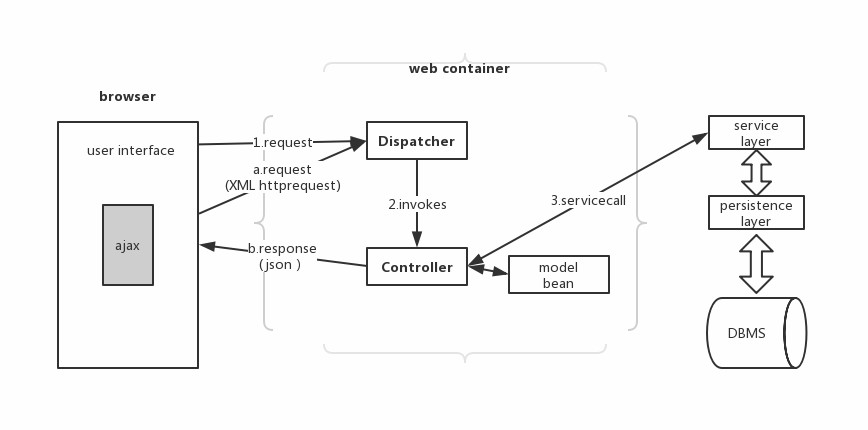
\includegraphics[width=1.0\linewidth]{figure/BS_structure}
	\label{fig:BS_structure}  \\
		4.1 B/S架构图
\end{figure}

\subsubsection{RESTful API}

REST全称是Representational State Transfer,中文意思是表述(编者注:通常译为表征)性状态转移。

RESTful API有以下的特征:

(1)每一个uri代表一种资源。

(2)客户端和服务器之间,传递这种资源的某种表现层。

(3)客户端通过四个HTTP动词(GET、POST、DELETE、PUT),对服务器端资源进行操作,实现"表现层状态转化"(增删改查)。

(4)URL中通常不出现动词,只有名词。

(5)使用JSON不使用XML。

\subsubsection{使用Redux存储网络请求状态}

Redux 是 JavaScript 状态容器,提供可预测化的状态管理。可以让你构建一致化的应用,运行于不同的环境(客户端、服务器、原生应用),并且易于测试。其使用Immutable数据结合React能让页面相应数据进行最小颗粒度的更新DOM结点。

redux数据流如图4.2所示

\begin{figure}[thbp!]
	\centering
	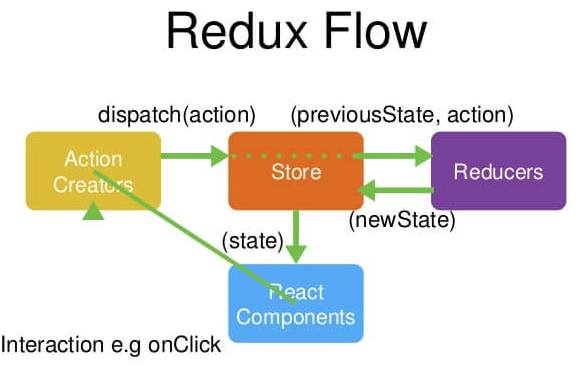
\includegraphics[width=1.0\linewidth]{figure/redux}
	\label{fig:redux} \\
		4.2 redux数据流
\end{figure}

每一次发起http请求获得响应的时候触发一个Redux Action,将服务端返回的数据存储在store中。这样做的好处是所有的需要使用服务端数据的React组件不需要影响父子组件之间的数据流直接提取公用的状态。

\subsection{账号系统}

\subsubsection{密码加密}

用户密码的创建和验证简略代码如下:

\begin{lstlisting}[language=C]
@property
def password(self):
raise TypeError("cannot read a user's password")

@password.setter
def password(self, password):
self.password_hash = generate_password_hash(password)

def verify_password(self, password):
if not password:
return False
return check_password_hash(self.password_hash, password)
\end{lstlisting}

@property装饰器装饰一个属性的getter,修饰的函数名为属性名,返回的值是该属性的getter,此处该属性不能直接访问访问则会抛出异常。

@property同时会全局创建一个@password.setter的装饰器装饰属性的setter,在设置password的时候我们其实设置的是password\_hash这个属性,值为hash加密过的password。

处理登陆请求的时候调用verify\_password函数判断密码是否正确。

这样做的好处就是即使是数据库管理员也不可能知道用户的密码,只能看到加密后的字符串,同时md5是不可逆的加密方式,不能由加密后的字符串反推出明文,保证了数据的机密性。

\subsubsection{邮箱验证}

用户注册和忘记密码的时候需要使用邮箱验证。在用户注册成功后会创建一个用户独有的token,将token作为链接参数发送给用户邮箱中,在用户点击链接进入验证页面的时候会将token返回后端后端进行验证。

验证失败有两种结果,一是token过期,二是token中的用户信息不匹配当前用户。通常不匹配的情况有三种:

(1) 用户自己改了url中的token

(2) 中间商劫持被修改了token信息。

(3) 非法重定向。

无论哪种都是非法篡改token的行为,影响用户信息安全。

邮箱激活流程图如图4.3所示,用户注册以后,系统会向注册时候填写的邮箱中发送一个邮件,里面带有验证地址的连接,用户点击以后进入验证页面。有两种用户,一种是自主创建的用户,一种是管理员批量添加的用户,第二种用户在登陆的时候需要填写邮箱,然后再进行激活。如果用户篡改连接地址或者被运营商劫持验证时不会通过。因为连接中有一个参数为token,token是将用户信息和时间戳hash后的可逆加密字符串,一旦服务端验证token的时候信息和连接中的username参数对不上那就会返回失败。

\begin{figure}[thbp!]
	\centering
	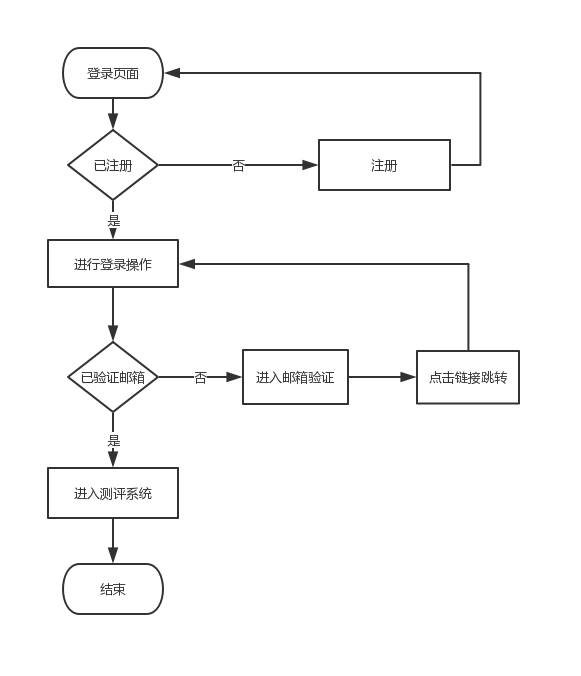
\includegraphics[width=1.0\linewidth]{figure/register_email}
	\label{fig:register_email} \\
		图4.3 注册邮箱激活
\end{figure}

找回密码流程图如图4.4所示,用户忘记密码后点击忘记密码,需要输入自己的用户名,随后系统会向用户名注册时候对应的邮箱发送验证邮箱,点击邮箱中的连接进入验证界面如果验证通过则会出现新密码输入框。

\begin{figure}[thbp!]
	\centering
	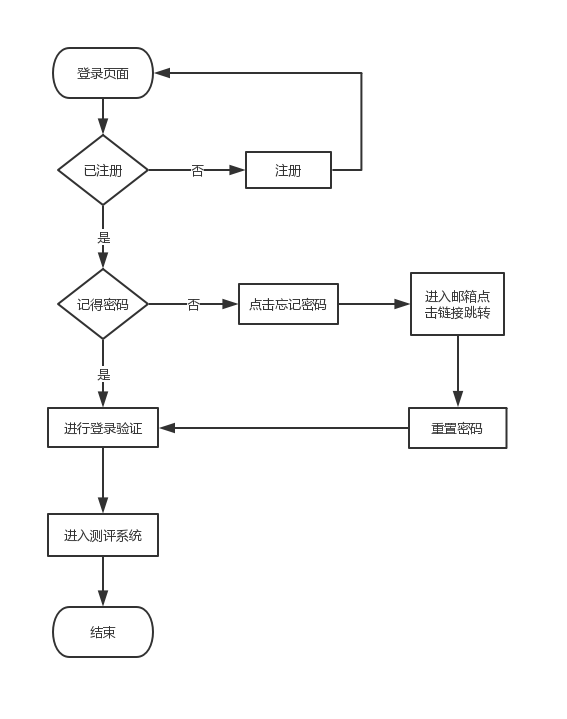
\includegraphics[width=0.8\linewidth]{figure/password_mail}
	\label{fig:password_email} \\
		图4.4 忘记密码邮箱验证
\end{figure}

\subsection{评测与数据分析}

\subsubsection{上传试卷}

示例试卷excel表格如图4.5所示

\begin{figure}[thbp!]
	\centering
	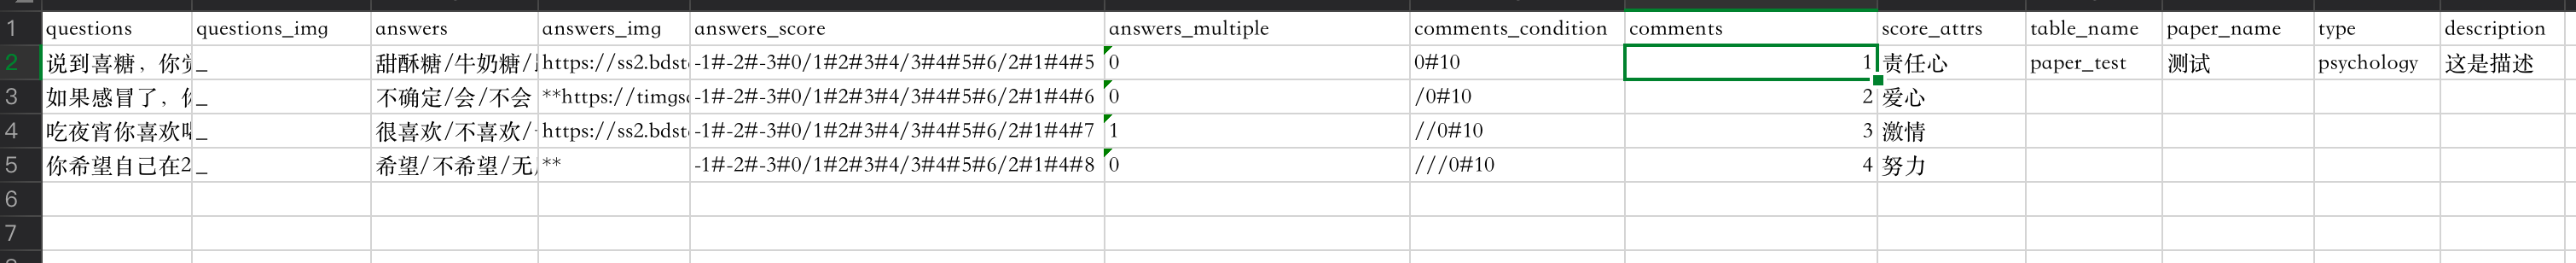
\includegraphics[width=1.0\linewidth]{figure/paper}
	\label{fig:paper} \\
		图4.5 示例试卷
\end{figure}

mysql中试卷表如图4.6所示

\begin{figure}[thbp!]
	\centering
	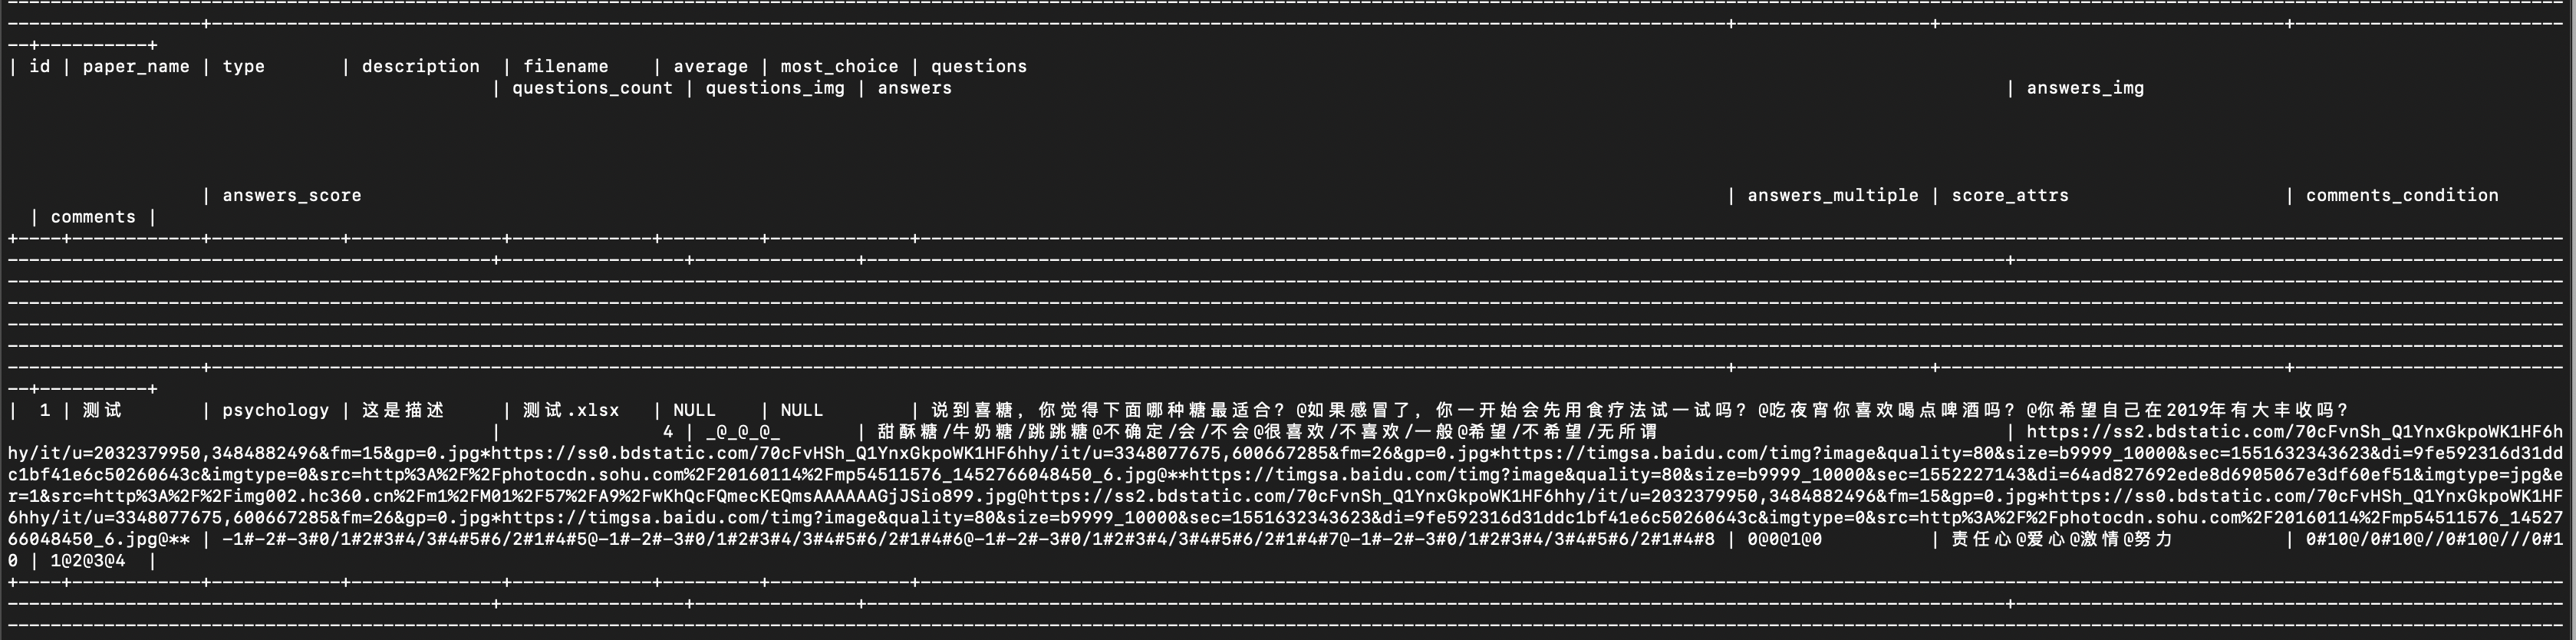
\includegraphics[width=1.0\linewidth]{figure/paper_database}
	\label{fig:paper_database} \\
		图4.6 试卷表
\end{figure}

上传试卷是通过上传excel表格。

questions 问题的题目

questions\_img 题目的配图的图片链接地址

answers 题目的答案,答案之间用"/"来进行分割

answers\_img 题目答案的配图的图片链接地址,配图之间用"*"进行分割,只支持一个答案只有一个配图

answers\_score 对应每个答案对应试卷指标的分数加成,正数为增加,负数为减少,0则表示该答案对此项指标没有影响,每个答案之间用"/"分隔,每个指标之间用"\#"分隔

answers\_multiple 该题目是否是多选,0表示单选,1表示多选

comments\_condition 试卷各种评论的条件,每个指标之间用"/"分隔,0\#10表示该指标大于零小于10

comments 具体的评论内容

score\_attrs 试卷的得分指标

table\_name 数据库中的表名

paper\_name 试卷名称

type 试卷的类型,psychology代表室心理评测,grade代表普通试卷,决定了试卷的算分机制

description 试卷的描述

上传文件后后端通过读取excel表格文件将数据插入到数据库中。

每个问题之间的数据使用"@"来进行连接。

在评测时候后端会对表数据进行解析和构建对象发送给前端。

试卷数据结构如图4.7所示

\begin{figure}[thbp!]
	\centering
	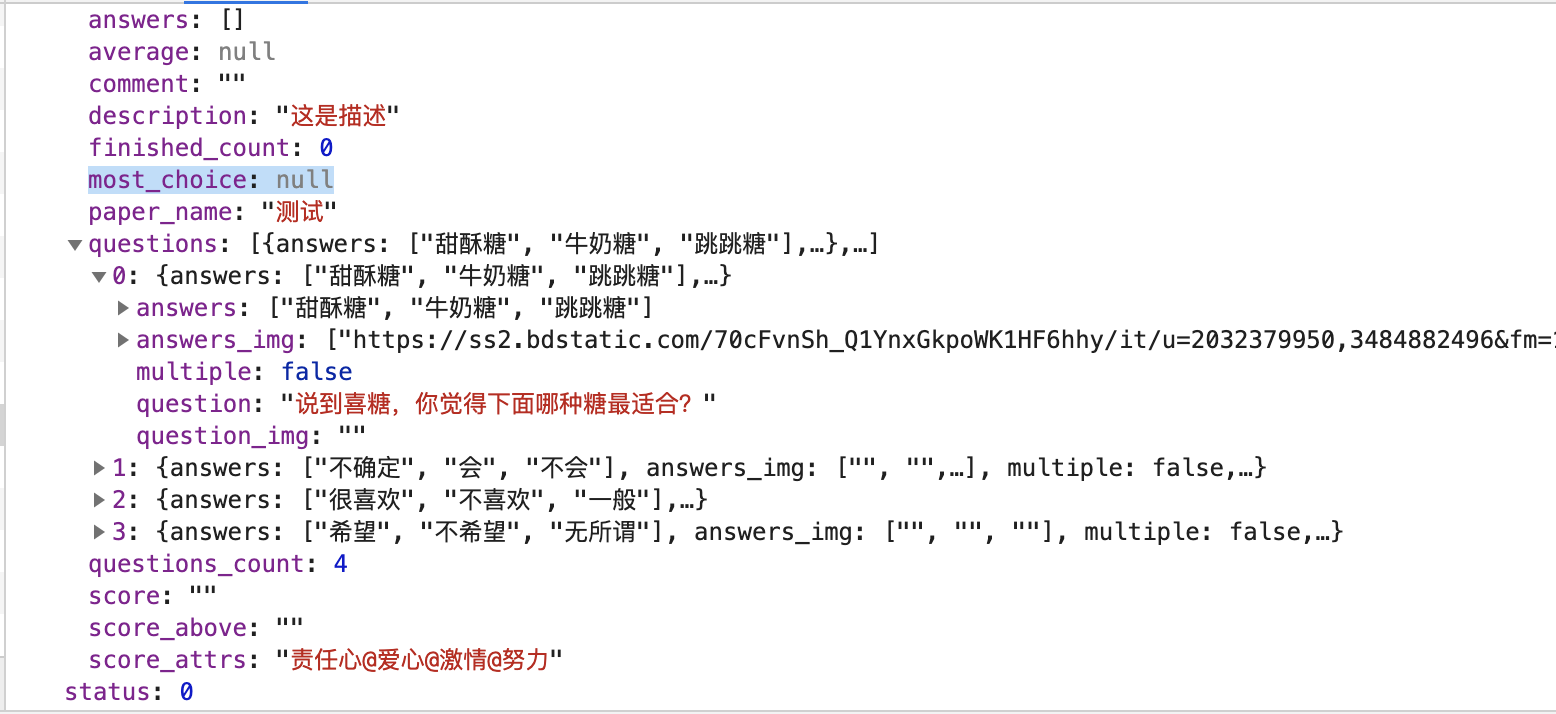
\includegraphics[width=1.0\linewidth]{figure/paper_data}
	\label{fig:paper_data} \\
		图4.7 试卷数据结构
\end{figure}

其中average、comment、most\_choices、answers、score、score\_above、score\_attrs是完成试卷以后才会有的参数,与数据分析结果的接口是一个接口。

\subsubsection{数据分析}

成绩数据表如图4.8所示

\begin{figure}[thbp!]
	\centering
	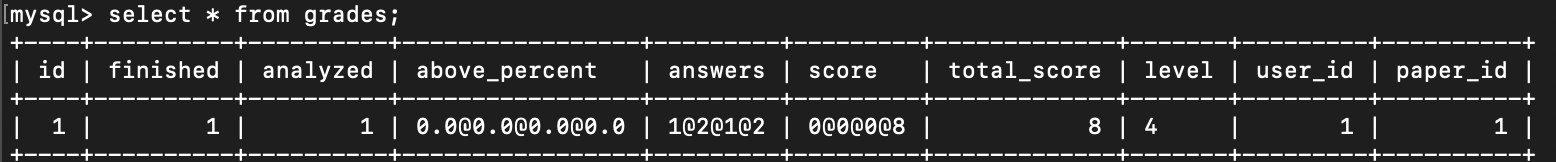
\includegraphics[width=1.0\linewidth]{figure/grade}
	\label{fig:grade} \\
		图4.8 成绩数据表
\end{figure}

用户回答完后,答案之间以"@"分隔开来进行存储。在计算得分的时候遍历答案进行指标的加减。

\subsubsection{计算每个问题最多回答的答案}

计算最多回答的答案的简略代码:

\begin{lstlisting}[language=C]
most_choice = "@".join(map(lambda x: Counter(x)
.most_common(1)[0][0], choices))
\end{lstlisting}

Counter是Python内置的一个计数器类,可以得到每个元素出现的次数,其中.most\_common函数可以得到列表中出现频率最频繁的元素。

%============= 参考文献 =====================
\section*{参考文献}
\addcontentsline{toc}{section}{参考文献}

[1] 未来科技. jQuery 实战从入门到精通 [M]. 水利水电出版社, 2017. 

[2] 叶维忠. Python 编程从入门到精通 [M]. 人民邮电出版社, 2017. 

[3] 杜文洁. 高等学校毕业设计(论文)指导教程——电子信息类专业 [M]. 水利水电出 版社, 2015. 

[4] 刘一奇. React 与 Redux 开发实例精解 [M], 2016. 

[5] 程墨. 深入浅出 React 和 Redux[M]. 机械工业出版社, 2017. 

[6] 程墨. 深入浅出 RxJS[M]. 机械工业出版社, 2018. 

[7] 张静. 慧眼识人——心理学评测在人才管理中的应用 [M]. 辽宁科技, 2016.

[8] 吴浩麟. 深入浅出 webpack[M]. 电子工业出版社, 2018. 

[9] Crockford. JavaScript:The Good Parts[M]. Southeast University Press, 2008. 

[10] BANKS A, PORCELLO E. Python 编程从入门到精通 [M]. China Electric Power Press, 2017. 

[11] JAWORSKI M, ZIADE T. Expert Python Programming[M]. PacktPublishing, 2016. 

[12] RAMALHO L. Fluent Python[M]. Posts and Telecommunications Press, 2017. 

[13] GORELICK M, OZSVALD I. High Performance Python[M]. Posts and Telecommunications Press, 2017. 

[14] Miguel Greenberg. Flask Web Development[M]. Posts and Telecommunications Press, 2018. 

[15] Gustave Le Bon. The crowd: a study of the popular mind[M]. Guangxi Normal University Press, 2011.
%=============  致谢  ======================
\section*{致谢}
\addcontentsline{toc}{section}{致谢}
四年的大学生活即将结束同时也代表着十六年的学生生涯也即将画上句号,但这只是我人生的开始,感谢父母孜孜不倦的教导和对我生活、学业、生活上的支持,也感谢这些年来老师勤勤恳恳耐心的教导。本系统设计与实现期间得到了我的导师刘传文的耐心指导,是刘老师让我明白学术的力量,营造了一种良好的学术氛围,让我的系统更加完善,论文更加严谨。历时一个学习的毕业设计,期间获得了许多同学和老师的帮助,在这里真挚的感谢你们。

\end{document}
%%%%%%%%%% 结束 %%%%%%%%%%